\documentclass{article}

% ----------------------------------------------------------------
% Packages
\usepackage{lipsum}
\usepackage[utf8]{inputenc}
\usepackage[style=ieee, defernumbers, backend=biber]{biblatex}
\usepackage[T1]{fontenc}
\usepackage{csquotes}
\usepackage{graphicx}
\usepackage{caption}                        % for captions
\usepackage[ngerman]{babel}                 % german language support
\usepackage[T1]{fontenc}                    % fix non asci letter encoding
\usepackage[nottoc,numbib]{tocbibind}       % for numbering list of figures
                                            % and images and equations
% \usepackage[titles]{tocloft}              % for custom list of equations
\usepackage[left=3cm,right=3cm]{geometry}   % make page wider
\usepackage{float}                          % reposition images and tables
\usepackage{epstopdf}                       % if using EPS format
\usepackage{amsmath}                        % for additional math symbols and environments
% ----------------------------------------------------------------

% ----------------------------------------------------------------
% Setup bibliography references style
\addbibresource{literatur.bib}
% ----------------------------------------------------------------

% ----------------------------------------------------------------
% Make my custom list of equations
% TODO!!!
% ----------------------------------------------------------------

% ----------------------------------------------------------------
% Add numbering to list of figures, list of tables
\renewcommand{\listoffigures}{%
    \begingroup
    \let\section\subsection % change section to be subsection
    \tocsection
    \tocfile{\listfigurename}{lof}
    \endgroup
}
\renewcommand{\listoftables}{%
    \begingroup
    \let\section\subsection % change section to be subsection
    \tocsection
    \tocfile{\listtablename}{lot}
    \endgroup
}
% ----------------------------------------------------------------

% ----------------------------------------------------------------
% Title, author and date
\title{
    \LARGE \textbf{Laborübung II}
    \vspace{0.5cm}
    \hrule height 2pt
    \vspace{0.5cm}
    \textbf{Laborprotokoll Drehpendel}
    \vspace{0.5cm}
    \hrule height 2pt
    \vspace*{15\baselineskip}
    {
        \small Gruppenmitglieder: Lucas Hörl und Rafał Dąbek
        \\
		Betreuer: Prof. Johann Laimer
    }

}
\author{
    \textbf{Rafał Dąbek}
}
\date{
    fertiggestellt am \today \\
    \textit{Versuchsdurchführung am 29. November 2023}
}
% ----------------------------------------------------------------

% ----------------------------------------------------------------
% Make links in the document
\usepackage{hyperref}                   % for links
% Setup links
\hypersetup{
    colorlinks,
    citecolor=black,
    filecolor=black,
    linkcolor=black,
    urlcolor=black
}
% ----------------------------------------------------------------

\begin{document}

% First page with title, author and date
\maketitle
\clearpage

% Second page with table of contents
\tableofcontents
\clearpage

\section{Einleitung}
Dieses Laborprotokoll befasst sich mit der Ausmessung charakteristischer Größen eines Drehpendels nach Pohl. Das Pohlsche Rad
ermöglicht die Bestimmung der Eigenschaften des Systems bei verschiedenen Dämpfungen und Erregerfrequenzen.
Die Versuche umfassen die Bestimmung der Eigenfrequenz des Systems, die Messung an freien und erzwungenen Schwingungen bei verschiedenen Dämpfungen,
sowie auch die Bestimmung einer Resonanzkurve.

\section{Theoretische Grundlagen des Pendels}
\subsection{Differentialgleichung}
Die mathematische Beschreibung des Pendels erfolgt über eine Gleichung der Drehmomente, welche durch die folgende
Differentialgleichung 2. Ordnung beschrieben werden kann:
\begin{gather} \label{eq:pendel}
    J \cdot \ddot \varphi(t) + r \cdot \dot \varphi(t) + D \cdot \varphi(t) = M_{0} \cdot cos(\omega_{E} \cdot t)
\end{gather}
Die einzelnen Terme stehen für:
\begin{flushleft}
\begin{tabular}{lc@{ }l}
    $\varphi(t)$ & ... & die Auslenkung (Winkel) des Pendels\\
    $\dot \varphi(t)$ & ... & die Winkelgeschwindigkeit des Pendels\\
    $\ddot \varphi(t)$ & ... & die Winkelbeschleunigung des Pendels\\
    $J$ & ... & das Trägheitsmoment des Pendelkörpers\\
    $r$ & ... & der Dämpfungskoeffizient (Wirbelstrombremse)\\
    $D$ & ... & die Winkelrichtgröße\\
    $M_{0}$ & ... & die Amplitude des Drehmoments des Erregers\\
    $\omega_{E}$ & ... & die Erregerfrequenz
\end{tabular}
\end{flushleft}
Das Trägheitsmoment wird definiert als $J = \rho \cdot \int_{V}^{} r^{2} dV$.
\cite{w:traegheit}

\subsection{Die Lösung der Differentialgleichung}
\subsubsection{Freie Schwingung}
Die freie Schwingung findet statt, wenn der Dämpfungsterm und Erregerterm wegfallen, d.h. $r = 0$ und $M_{0} = 0$.
Die Differentialgleichung lautet dann:
\begin{gather} \label{eq:freie_schwingung}
    J \cdot \ddot \varphi(t) + D \cdot \varphi(t) = 0\\
    \ddot \varphi(t) + \frac{D}{J} \cdot \varphi(t) = 0
\end{gather}
Die Lösung erfolgt durch den Exponentialansatz:
\begin{gather} \label{eq:freie_schwingung_ansatz}
    \varphi(t) = A \cdot e^{\lambda \cdot t}\\
    \ddot \varphi(t) = \lambda^{2} \cdot A \cdot e^{\lambda \cdot t}
\end{gather}
Dadurch entsteht die charakteristische Gleichung:
\begin{gather} \label{eq:freie_schwingung_char_gl}
    \lambda^{2} + \lambda \cdot \frac{D}{J} = 0\\
    \lambda = \pm i \cdot \sqrt{\frac{D}{J}}
\end{gather}
Sehr praktisch ist hier $\omega_{0}$ zu definieren als $\omega_{0} = \sqrt{\frac{D}{J}}$, bzw. $\omega_{0}^{2} = \frac{D}{J}$.
Somit ist $\lambda = \pm i \cdot \omega_{0}$. Die Lösung ist dann
$\varphi(t) = A_{1} \cdot e^{-i \omega_{0} \cdot t} + A_{2} \cdot e^{i \omega_{0} \cdot t}$.
Durch die Eulersche Identität $e^{i \cdot \varphi} = cos(\varphi) + i \cdot sin(\varphi)$ kann auf die Form
$\varphi(t) = B_{1} \cdot cos(\omega_{0} \cdot t) + B_{2} \cdot sin(\omega_{0} \cdot t)$ umgeformt werden. Mit den Anfangsbedingungen
\begin{gather} \label{eq:freie_schwingung_anfangsbed}
    \varphi(t = 0) = \varphi_{0}\\
    \dot \varphi(t = 0) = 0
\end{gather}
ergibt sich die Lösung:
\begin{gather} \label{eq:freie_schwingung_loesung}
    \varphi(t) = \varphi_{0} \cdot cos(\omega_{0} \cdot t)
\end{gather}
\subsubsection{Gedämpfte Schwingung}

\begin{figure}[H]
    \centering
    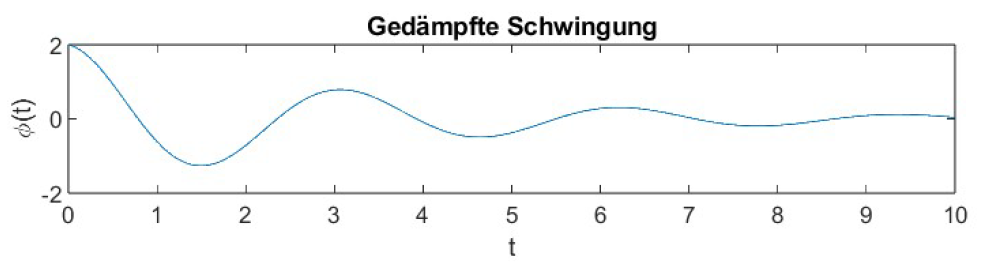
\includegraphics[width=0.6\textwidth]{bilder/schwingung_gedampft.png}
    \caption{Gedämpfte Schwingung}
    \label{fig:schw_ged}
\end{figure}

\subsubsection{Aperiodischer Grenzfall}

\begin{figure}[H]
    \centering
    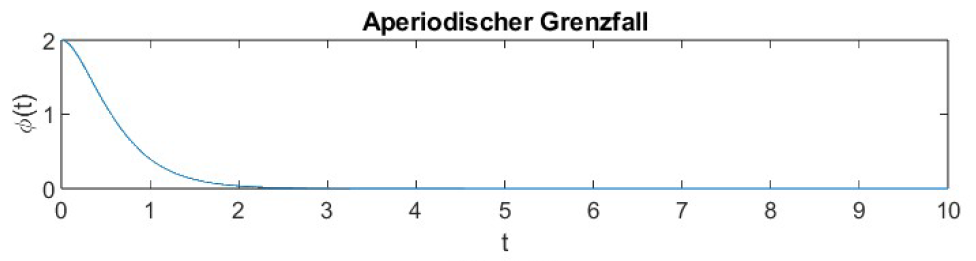
\includegraphics[width=0.6\textwidth]{bilder/aperiodischer_grenzfall.png}
    \caption{Aperiodischer Grenzfall}
    \label{fig:aperiod}
\end{figure}

\subsubsection{Kriechfall}

\begin{figure}[H]
    \centering
    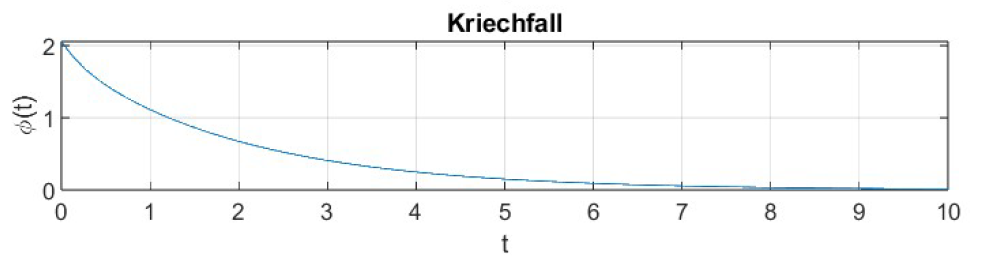
\includegraphics[width=0.6\textwidth]{bilder/kriechfall.png}
    \caption{Kriechfall}
    \label{fig:kriech}
\end{figure}

\subsection{Die Lösung der inhomogenen Differentialgleichung}
\subsubsection{Resonanzkurven}

\section{Versuchsaufbau}
Der Versuchsaufbau bestand aus einem Drehpendel nach Pohl der Firma Leybold \ref{fig:versuchsaufbau}.
Für die Messungen stand das Programm CASSY auf einem Labor-PC zur Verfügung.
Das Messystem erfasste automatisch über die entsprechende Schnittstellen \ref{fig:schnittstelle}
nach dem Start einer Aufzeichnung die Bewegung des Pendelkörpers
über den BMW (Bewegungsmesswandler). Diese Daten wurden dann in der CASSY-Software
und in Microsoft Excel ausgewertet.

\begin{figure}[H]
    \centering
    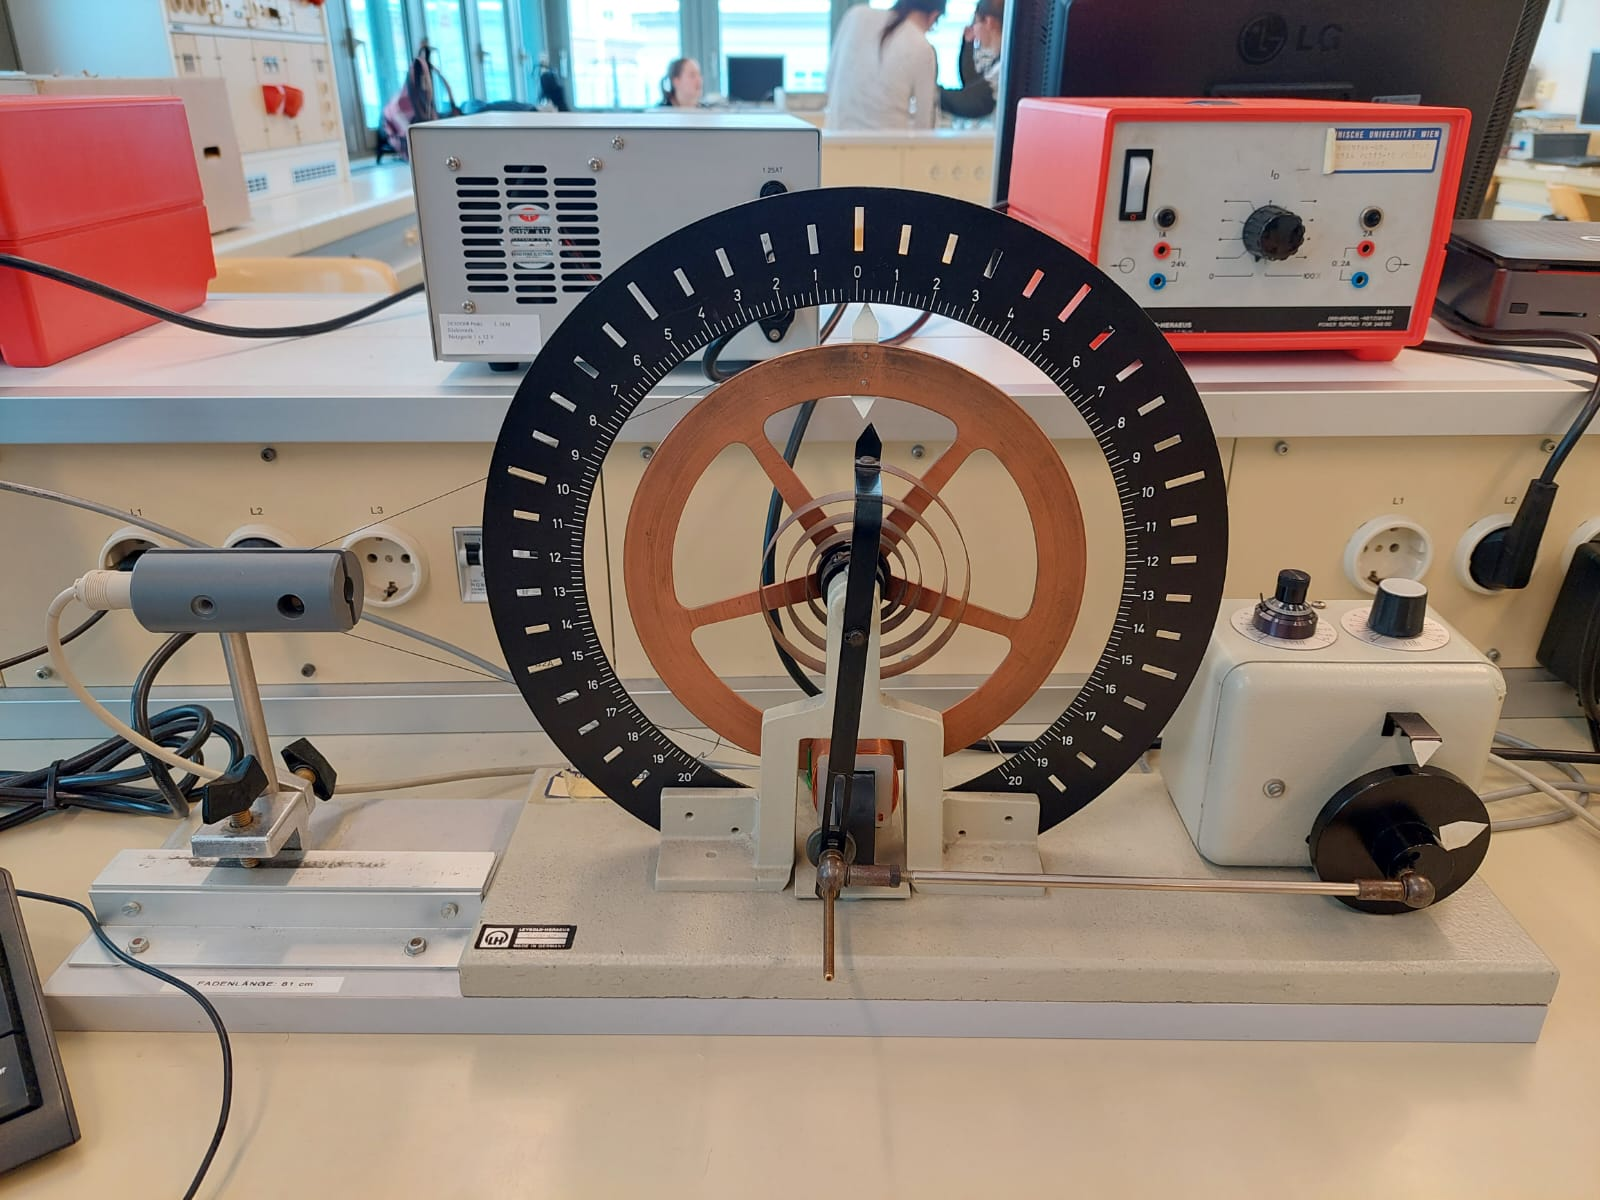
\includegraphics[width=0.6\textwidth]{bilder/drehpendel.jpg}
    \caption{Ein Foto des Versuchsaufbaus}
    \label{fig:versuchsaufbau}
\end{figure}

\begin{figure}[H]
    \centering
    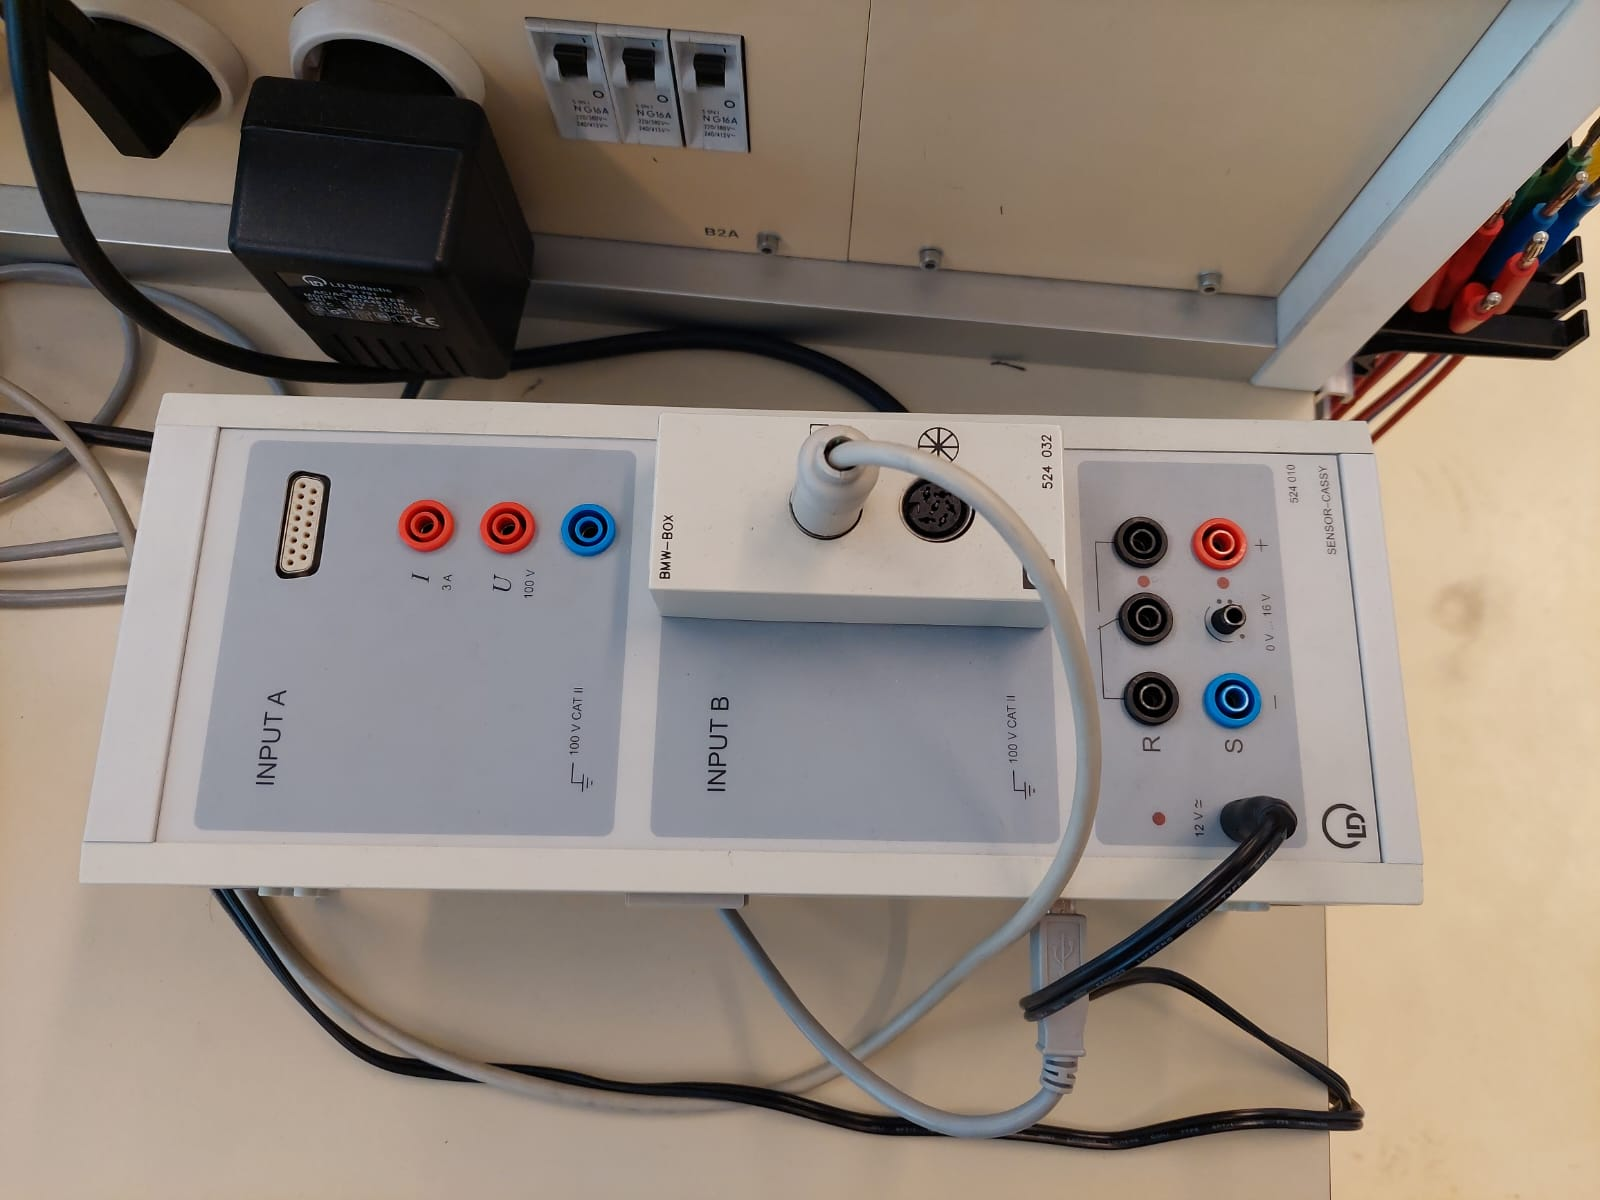
\includegraphics[width=0.6\textwidth]{bilder/sensor_cassy.jpg}
    \caption{Ein Foto der Schnittstelle}
    \label{fig:schnittstelle}
\end{figure}

Der Aufbau des Pendels \cite{w:pohl} besteht aus einem Kupferrad, welches das Pendel simulieren soll.
Das Kupferrad ist über eine Nabe an eine Feder verbunden. Diese bewirkt das entsprechende
Rückstellmoment. Außerdem kann das Pendel über einen Hebel, der exzentrisch an einem
elektrischen Motor befestigt ist, angetrieben werden. Letzendlich kann mit einer Wirbelstrombremse
eine zusätzliche Dämpfung eingestellt werden.

\begin{figure}[H]
    \centering
    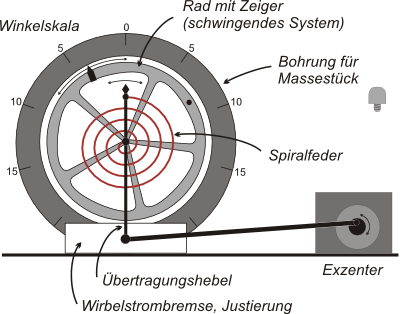
\includegraphics[width=0.6\textwidth]{bilder/drehpendel_pohl.png}
    \caption{Das Pendel nach Pohl \cite{w:pohl_drehpendel}}
    \label{fig:pendel}
\end{figure}

\section{Versuche}
\subsection{Bestimmung der Eigenfrequenz} \label{ssec:eigenfrequenz}
\subsubsection{Durchführung}
Das Ziel dieses Versuches war es die Eigenfrequenz $f$ und die Abklingkonstante $\delta$ zu
bestimmen. Die Dämpfung sollte dabei nicht vorhanden sein, d.h. die Wirbelstrombremse
sollte ausgeschaltet bleiben. Die Bestimmung der Eigenfrequenz erfolgte über
die Messung der Zeit $\Delta t$ über mehrere Perioden n. Die Frequenz wird dann
folgendermaßen berechnet: $f = \frac{n}{\Delta t}$.

Die Abklingkonstante $\delta$ konnte mittels CASSY aus dem Wert $B$ folgend
bestimmt werden: $\delta = \frac{1}{B}$, wobei $B$ aus der Messung abgelesen werden konnte. $B$ berechnet CASSY aus der
Einhüllenden der Schwingung.

Das Dämpfungsdekrement $k$ wird über die Formel $k^n = \frac{A_1}{A_{n+1}}$ bestimmt. Die Abklingskonstante $\delta$ ist
mit dem Dämpfungsdekrement $k$ folgend verknüpft: $\delta = \frac{ln(k)}{T}$.
\subsubsection{Messdaten}
\begin{table}[H]
    \centering
    \begin{tabular}{|c|c|c|c|c|c|c|c|c|}
    \hline
    $\Delta t$ (s) & $n$ & $T$ (s) & $f$ (Hz) & $A_{n+1}$ (rad) & $A_1$ (rad) & $B$ (s) & $\delta_{CASSY}$ (s) & k\\
    \hline
    5.23 & 3 & 1.740 & 0.574 & 0.19 & 0.45 & 6.19 & 0.16 & 0.75 \\
    5.15 & 3 & 1.717 & 0.583 & 0.18 & 0.43 & 6.27 & 0.16 & 0.75 \\
    5.11 & 3 & 1.703 & 0.587 & 0.16 & 0.42 & 5.56 & 0.18 & 0.73 \\
    5.16 & 3 & 1.720 & 0.581 & 0.18 & 0.43 & 6.28 & 0.16 & 0.75 \\
    5.14 & 3 & 1.713 & 0.584 & 0.18 & 0.44 & 6.60 & 0.15 & 0.74 \\
    5.11 & 3 & 1.703 & 0.587 & 0.19 & 0.44 & 6.79 & 0.15 & 0.76 \\
    \hline
    \end{tabular}
    \caption{Bestimmung der Eigenfrequenz}
    \label{tab:eigenfrequenz}
\end{table}

\begin{figure}[H]
    \centering
    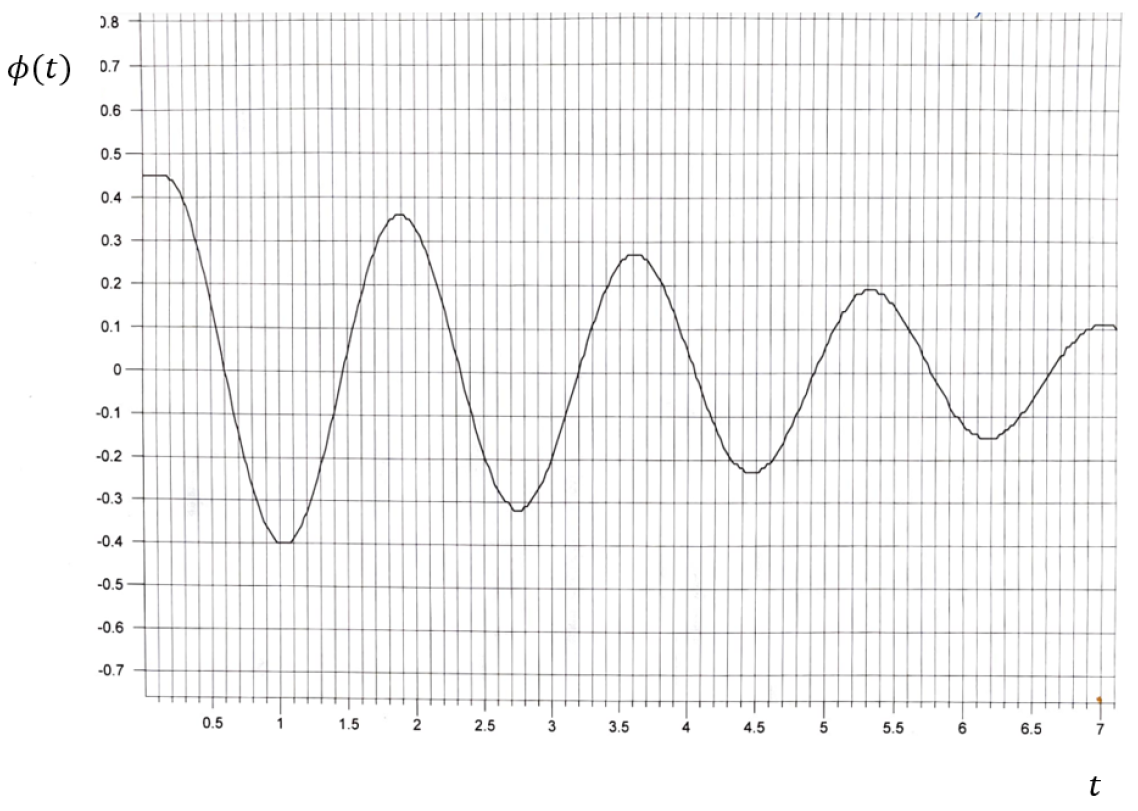
\includegraphics[width=0.6\textwidth]{bilder/eigenfreq_messdaten.png}
    \caption{Messung des Auslenkwinkels $\phi(t)$ in CASSY}
    \label{fig:eigenfreq_messdaten}
\end{figure}

\begin{figure}[H]
    \centering
    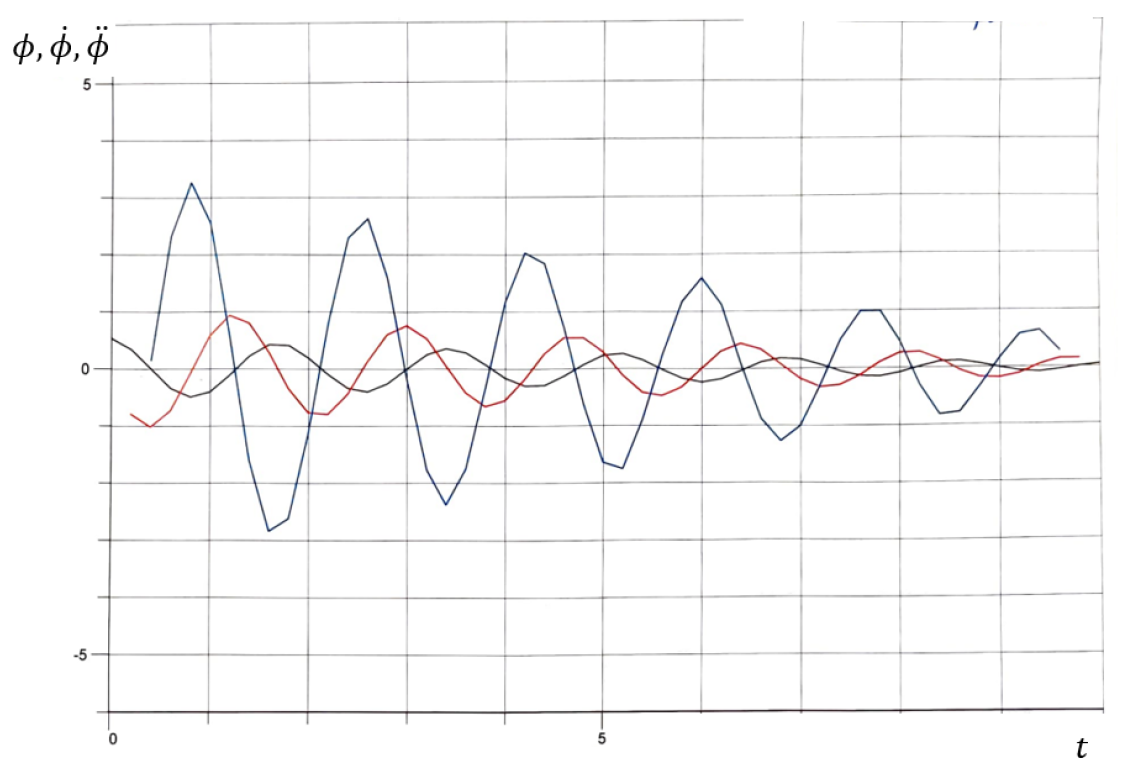
\includegraphics[width=0.6\textwidth]{bilder/eigenfreq_ableitungen_messdaten.png}
    \caption{Messung des Auslenkwinkels $\phi(t)$ (schwarz) und der Ableitungen $\dot\phi(t)$ (rot) und $\ddot\phi(t)$ (blau) in CASSY}
    \label{fig:eigenfreq_abl_messdaten}
\end{figure}

\subsubsection{Diskussion}
Der Mittelwert von $T$ ergibt sich aus der Tabelle \ref{tab:schwingung_dämpfungen} als $T = 1.716 \pm 0.014s$. Somit ergibt sich $f$ unter Berücksichtigung der
Fehlerforpflantzung als $0.583 \pm 0.005Hz$. Für das Dämpfungsdekrement $k$ folgt $k = 0.75 \pm 0.01$. Somit beträgt die Abklingkonstante $\delta = 0.17 \pm 0.01s^{-1}$.
Außerdem folgt auch $\delta_{CASSY} = 0.17 \pm 0.01s^{-1}$.

Es ist somit ersichtlich, dass die beiden Werte recht gut übereinstimmen. Sowohl der händisch berechnete Wert, als auch der von CASSY bestimmte Wert liegen in Grenzen der
Standardabeichung.

\subsection{Schwingung bei verschiedenen Dämpfungen}
\subsubsection{Durchführung}

\subsubsection{Messdaten}
\begin{table}[H]
    \centering
    \begin{tabular}{|c|c|c|c|c|c|c|c|}
    \hline
    $I$ (mA) & $n$ & $A_1$ (rad) & $A_n$ (rad) & $B$ (s) & $\delta_{CASSY}$ (s$^{-1}$) & $\Delta t$ (s) & $T$ (s) \\
    \hline
    351 & 3 & 0.57 & 0.32 & 4.43 & 0.23 & 5.17 & 0.58 \\
    349 & 3 & 0.54 & 0.33 & 4.30 & 0.23 & 5.15 & 0.58 \\
    348 & 3 & 0.54 & 0.29 & 4.37 & 0.23 & 5.21 & 0.58 \\
    596 & 2 & 0.55 & 0.22 & 2.35 & 0.43 & 3.47 & 0.58 \\
    590 & 2 & 0.55 & 0.23 & 2.61 & 0.38 & 3.45 & 0.58 \\
    593 & 2 & 0.55 & 0.19 & 2.59 & 0.39 & 3.47 & 0.58 \\
    900 & 2 & 0.56 & 0.03 & 1.00 & 1.00 & 3.41 & 1.71 \\
    901 & 2 & 0.55 & 0.03 & 1.14 & 0.88 & 3.39 & 1.70 \\
    898 & 2 & 0.57 & 0.03 & 0.99 & 1.01 & 3.44 & 1.72 \\
    1486 & 1 & 0.56 & 0.01 & / & / & 1.90 & 1.90 \\
    \hline
    \end{tabular}
    \caption{Schwingungen bei verschiedenen Dämpfungen}
    \label{tab:schwingung_dämpfungen}
\end{table}

\begin{table}[H]
    \centering
    \begin{tabular}{|c|c|c|c|}
    \hline
    $I$ (mA) & $\delta_{CASSY}$ (s$^{-1}$) & $\delta$ (s$^{-1}$) \\
    \hline
    0 & $0.16 \pm 0.01$ & $0.17 \pm 0.01$ \\
    $350 \pm 3$ & $0.23 \pm 0.01$ & $0.32 \pm 0.04$ \\
    $595 \pm 3$ & $0.40 \pm 0.02$ & $0.82 \pm 0.07$ \\
    $900 \pm 3$ & $0.76 \pm 0.26$ & $0.86 \pm 0.01$ \\
    $1486 \pm 3$ & / & $2.12 \pm 0.3$ \\
    \hline
    \end{tabular}
    \caption{Abklingskonstante $\delta_{CASSY}$ vs. $\delta$ händisch gerechnet beim Strom $I$}
    \label{tab:dämpfungen_strom}
\end{table}

\subsubsection{Diskussion}


\subsection{Zusammenhang Erregerfrequenz und Erregerspannung}
\subsubsection{Durchführung}
Das Ziel dieses Experimentes ist die Ermittlung des Zusammenhangs zwischen Erregerfreqzenz und Erregerspannung.
Dazu wurde die Spannung am Elektomotor variiert und die Frequenz des Systems bei jeder Spannung einzeln ausgemessen.
Das Messen der Frequenz erfolgt genauso wie in Abschnitt \ref{ssec:eigenfrequenz} beschrieben.

\subsubsection{Messdaten}
\begin{table}[H]
    \centering
    \begin{tabular}{|c|c|c|c|c|}
    \hline
    $U$ (V) & $f$ (Hz) & $\Delta t$ (s) & $n$ & $T$ (s) \\
    \hline
    6.00 & 0.43 & 6.98 & 3 & 2.33 \\
    7.00 & 0.53 & 7.60 & 4 & 1.90 \\
    8.00 & 0.62 & 8.11 & 5 & 1.62 \\
    9.00 & 0.68 & 8.80 & 6 & 1.47 \\
    9.99 & 0.80 & 8.71 & 7 & 1.24 \\
    11.01 & 0.89 & 9.00 & 8 & 1.13 \\
    11.98 & 0.98 & 8.20 & 8 & 1.03 \\
    12.99 & 1.07 & 8.39 & 9 & 0.93 \\
    14.00 & 1.17 & 8.55 & 10 & 0.86 \\
    15.00 & 1.26 & 8.75 & 11 & 0.80 \\
    \hline
    \end{tabular}
    \caption{Messung der Erregerfrequenzen und Erregerspannungen}
    \label{tab:messung_erregerfrequenz_spannung}
\end{table}

\begin{table}[H]
    \centering
    \begin{tabular}{|c|c|}
    \hline
    $U$ (V) $\pm$ 0.05 & $f$ (Hz) $\pm$ 0.01 \\
    \hline
    $6.00 \pm 0.05$ & $0.43 \pm 0.01$ \\
    $7.00 \pm 0.05$ & $0.53 \pm 0.01$ \\
    $8.00 \pm 0.05$ & $0.62 \pm 0.01$ \\
    $9.00 \pm 0.05$ & $0.68 \pm 0.01$ \\
    $9.99 \pm 0.05$ & $0.80 \pm 0.02$ \\
    $11.01 \pm 0.05$ & $0.89 \pm 0.02$ \\
    $11.98 \pm 0.05$ & $0.98 \pm 0.02$ \\
    $12.99 \pm 0.05$ & $1.07 \pm 0.02$ \\
    $14.00 \pm 0.05$ & $1.17 \pm 0.02$ \\
    $15.00 \pm 0.05$ & $1.26 \pm 0.03$ \\
    \hline
    \end{tabular}
    \caption{Zusammenhang Erregerfrequenz und Erregerspannung}
    \label{tab:erregerfrequenz_spannung}
\end{table}

\begin{figure}[H]
    \centering
    % GNUPLOT: LaTeX picture with Postscript
\begingroup
  % Encoding inside the plot.  In the header of your document, this encoding
  % should to defined, e.g., by using
  % \usepackage[cp1252,<other encodings>]{inputenc}
  \inputencoding{cp1252}%
  \makeatletter
  \providecommand\color[2][]{%
    \GenericError{(gnuplot) \space\space\space\@spaces}{%
      Package color not loaded in conjunction with
      terminal option `colourtext'%
    }{See the gnuplot documentation for explanation.%
    }{Either use 'blacktext' in gnuplot or load the package
      color.sty in LaTeX.}%
    \renewcommand\color[2][]{}%
  }%
  \providecommand\includegraphics[2][]{%
    \GenericError{(gnuplot) \space\space\space\@spaces}{%
      Package graphicx or graphics not loaded%
    }{See the gnuplot documentation for explanation.%
    }{The gnuplot epslatex terminal needs graphicx.sty or graphics.sty.}%
    \renewcommand\includegraphics[2][]{}%
  }%
  \providecommand\rotatebox[2]{#2}%
  \@ifundefined{ifGPcolor}{%
    \newif\ifGPcolor
    \GPcolortrue
  }{}%
  \@ifundefined{ifGPblacktext}{%
    \newif\ifGPblacktext
    \GPblacktexttrue
  }{}%
  % define a \g@addto@macro without @ in the name:
  \let\gplgaddtomacro\g@addto@macro
  % define empty templates for all commands taking text:
  \gdef\gplbacktext{}%
  \gdef\gplfronttext{}%
  \makeatother
  \ifGPblacktext
    % no textcolor at all
    \def\colorrgb#1{}%
    \def\colorgray#1{}%
  \else
    % gray or color?
    \ifGPcolor
      \def\colorrgb#1{\color[rgb]{#1}}%
      \def\colorgray#1{\color[gray]{#1}}%
      \expandafter\def\csname LTw\endcsname{\color{white}}%
      \expandafter\def\csname LTb\endcsname{\color{black}}%
      \expandafter\def\csname LTa\endcsname{\color{black}}%
      \expandafter\def\csname LT0\endcsname{\color[rgb]{1,0,0}}%
      \expandafter\def\csname LT1\endcsname{\color[rgb]{0,1,0}}%
      \expandafter\def\csname LT2\endcsname{\color[rgb]{0,0,1}}%
      \expandafter\def\csname LT3\endcsname{\color[rgb]{1,0,1}}%
      \expandafter\def\csname LT4\endcsname{\color[rgb]{0,1,1}}%
      \expandafter\def\csname LT5\endcsname{\color[rgb]{1,1,0}}%
      \expandafter\def\csname LT6\endcsname{\color[rgb]{0,0,0}}%
      \expandafter\def\csname LT7\endcsname{\color[rgb]{1,0.3,0}}%
      \expandafter\def\csname LT8\endcsname{\color[rgb]{0.5,0.5,0.5}}%
    \else
      % gray
      \def\colorrgb#1{\color{black}}%
      \def\colorgray#1{\color[gray]{#1}}%
      \expandafter\def\csname LTw\endcsname{\color{white}}%
      \expandafter\def\csname LTb\endcsname{\color{black}}%
      \expandafter\def\csname LTa\endcsname{\color{black}}%
      \expandafter\def\csname LT0\endcsname{\color{black}}%
      \expandafter\def\csname LT1\endcsname{\color{black}}%
      \expandafter\def\csname LT2\endcsname{\color{black}}%
      \expandafter\def\csname LT3\endcsname{\color{black}}%
      \expandafter\def\csname LT4\endcsname{\color{black}}%
      \expandafter\def\csname LT5\endcsname{\color{black}}%
      \expandafter\def\csname LT6\endcsname{\color{black}}%
      \expandafter\def\csname LT7\endcsname{\color{black}}%
      \expandafter\def\csname LT8\endcsname{\color{black}}%
    \fi
  \fi
    \setlength{\unitlength}{0.0500bp}%
    \ifx\gptboxheight\undefined%
      \newlength{\gptboxheight}%
      \newlength{\gptboxwidth}%
      \newsavebox{\gptboxtext}%
    \fi%
    \setlength{\fboxrule}{0.5pt}%
    \setlength{\fboxsep}{1pt}%
    \definecolor{tbcol}{rgb}{1,1,1}%
\begin{picture}(7200.00,5040.00)%
    \gplgaddtomacro\gplbacktext{%
      \csname LTb\endcsname%%
      \put(814,704){\makebox(0,0)[r]{\strut{}$0.4$}}%
      \csname LTb\endcsname%%
      \put(814,1161){\makebox(0,0)[r]{\strut{}$0.5$}}%
      \csname LTb\endcsname%%
      \put(814,1618){\makebox(0,0)[r]{\strut{}$0.6$}}%
      \csname LTb\endcsname%%
      \put(814,2076){\makebox(0,0)[r]{\strut{}$0.7$}}%
      \csname LTb\endcsname%%
      \put(814,2533){\makebox(0,0)[r]{\strut{}$0.8$}}%
      \csname LTb\endcsname%%
      \put(814,2990){\makebox(0,0)[r]{\strut{}$0.9$}}%
      \csname LTb\endcsname%%
      \put(814,3447){\makebox(0,0)[r]{\strut{}$1$}}%
      \csname LTb\endcsname%%
      \put(814,3905){\makebox(0,0)[r]{\strut{}$1.1$}}%
      \csname LTb\endcsname%%
      \put(814,4362){\makebox(0,0)[r]{\strut{}$1.2$}}%
      \csname LTb\endcsname%%
      \put(814,4819){\makebox(0,0)[r]{\strut{}$1.3$}}%
      \csname LTb\endcsname%%
      \put(946,484){\makebox(0,0){\strut{}$6$}}%
      \csname LTb\endcsname%%
      \put(1597,484){\makebox(0,0){\strut{}$7$}}%
      \csname LTb\endcsname%%
      \put(2248,484){\makebox(0,0){\strut{}$8$}}%
      \csname LTb\endcsname%%
      \put(2898,484){\makebox(0,0){\strut{}$9$}}%
      \csname LTb\endcsname%%
      \put(3549,484){\makebox(0,0){\strut{}$10$}}%
      \csname LTb\endcsname%%
      \put(4200,484){\makebox(0,0){\strut{}$11$}}%
      \csname LTb\endcsname%%
      \put(4851,484){\makebox(0,0){\strut{}$12$}}%
      \csname LTb\endcsname%%
      \put(5501,484){\makebox(0,0){\strut{}$13$}}%
      \csname LTb\endcsname%%
      \put(6152,484){\makebox(0,0){\strut{}$14$}}%
      \csname LTb\endcsname%%
      \put(6803,484){\makebox(0,0){\strut{}$15$}}%
    }%
    \gplgaddtomacro\gplfronttext{%
      \csname LTb\endcsname%%
      \put(209,2761){\rotatebox{-270}{\makebox(0,0){\strut{}$f$ (Hz)}}}%
      \put(3874,154){\makebox(0,0){\strut{}$U$ (V)}}%
      \csname LTb\endcsname%%
      \put(4642,4646){\makebox(0,0)[r]{\strut{}Messpunkte mit Fehlerbalken}}%
      \csname LTb\endcsname%%
      \put(4642,4426){\makebox(0,0)[r]{\strut{}$f(U)$}}%
    }%
    \gplbacktext
    \put(0,0){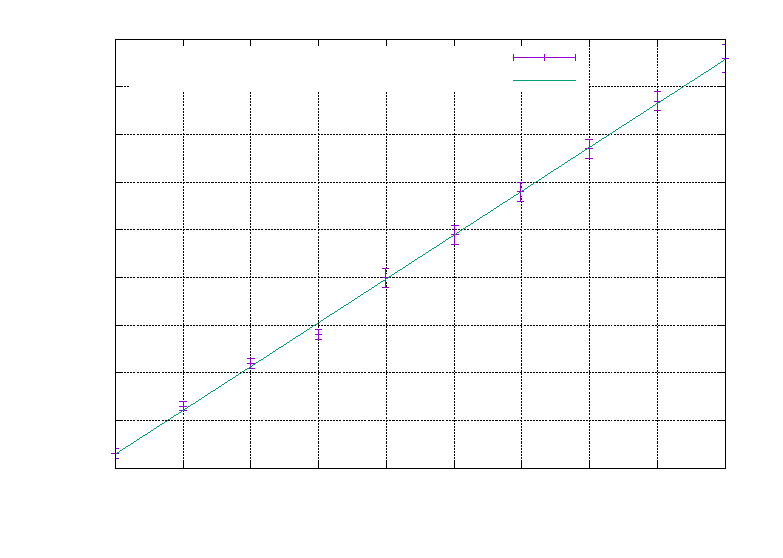
\includegraphics[width={360.00bp},height={252.00bp}]{bilder/erregerfrequenz_erregerspannung_linear_fit}}%
    \gplfronttext
  \end{picture}%
\endgroup

    \caption{Erregerfrequenz zu Erregerspannung mit linearem Fit $f(U)$}
    \label{fig:erreger_fit}
\end{figure}

In Abbildung \ref{fig:erreger_fit} wird der Zusammenhang mit der Funktion $f(U) = 0.092 \cdot U - 0.1239$ approximiert.

\subsubsection{Diskussion}
Die Ungenauigkeit bei der Spannung wurde mit $\sigma_{U} = 0.05 V$ angenommen. Mit der Fehlerforpflantzung wurden dann die
Ungenauigkeiten für die Frequenzen berechnet.
Es zeigt sich in Abbildung \ref{fig:erreger_fit}, dass der Zusammenhang zwischen Erregerfrequenz und Erregerspannung sehr gut linear approximiert
werden kann. Es gibt zwar einen Ausreißer, aber diesen erkläre ich mir über die Messungenauigkeit.

\subsection{Resonanzkurve}
\subsubsection{Durchführung}
Für die Bestimmung der Resonanzkurve ist es notwendig eine Dämpfung einzustellen. Die Dämpfung soll idealerweise so gewählt werden,
dass eine Resonanzkatastrophe vermieden wird. Danach wird der Drehwinkel des Pendels bei verschiedenen Erregerspannungen $U$ ausgemessen.
Für die Dämpfung wurde der Strom der Wirbelstrombremse $I = 610 mA$ gewählt. Über den annähernd linearen Zusammenhang der Erregerfrequenz
und Erregerspannung kann die Resonanzkurve bestimmt werden.

\subsubsection{Messdaten}
\begin{table}[H]
    \centering
    \begin{tabular}{|c|c|c|c|c|}
    \hline
    $I$ (mA) $\pm$ 3 & $U$ (V) $\pm$ 0.05 & $\varphi_{\text{max, pp}}$ (rad) $\pm$ 0.01 & $\varphi_{\text{max}}$ (rad) $\pm$ 0.005 & $f$ (Hz) $\pm$ 0.01 \\
    \hline
    $610 \pm 3$ & $5.99 \pm 0.05$ & $0.18 \pm 0.01$ & $0.090 \pm 0.005$ & $0.44 \pm 0.01$ \\
    $610 \pm 3$ & $7.00 \pm 0.05$ & $0.32 \pm 0.01$ & $0.160 \pm 0.005$ & $0.52 \pm 0.01$ \\
    $610 \pm 3$ & $8.00 \pm 0.05$ & $0.35 \pm 0.01$ & $0.175 \pm 0.005$ & $0.63 \pm 0.01$ \\
    $610 \pm 3$ & $9.00 \pm 0.05$ & $0.18 \pm 0.01$ & $0.090 \pm 0.005$ & $0.72 \pm 0.01$ \\
    $610 \pm 3$ & $9.99 \pm 0.05$ & $0.12 \pm 0.01$ & $0.060 \pm 0.005$ & $0.82 \pm 0.01$ \\
    $610 \pm 3$ & $5.00 \pm 0.05$ & $0.13 \pm 0.01$ & $0.065 \pm 0.005$ & $0.35 \pm 0.01$ \\
    $610 \pm 3$ & $6.50 \pm 0.05$ & $0.22 \pm 0.01$ & $0.110 \pm 0.005$ & $0.48 \pm 0.01$ \\
    $610 \pm 3$ & $7.50 \pm 0.05$ & $0.48 \pm 0.01$ & $0.240 \pm 0.005$ & $0.58 \pm 0.01$ \\
    $610 \pm 3$ & $8.50 \pm 0.05$ & $0.26 \pm 0.01$ & $0.130 \pm 0.005$ & $0.67 \pm 0.01$ \\
    $610 \pm 3$ & $7.25 \pm 0.05$ & $0.40 \pm 0.01$ & $0.200 \pm 0.005$ & $0.55 \pm 0.01$ \\
    $610 \pm 3$ & $8.25 \pm 0.05$ & $0.31 \pm 0.01$ & $0.155 \pm 0.005$ & $0.65 \pm 0.01$ \\
    $610 \pm 3$ & $8.10 \pm 0.05$ & $0.35 \pm 0.01$ & $0.175 \pm 0.005$ & $0.63 \pm 0.01$ \\
    \hline
    \end{tabular}
    \caption{Resonanzkurve}
    \label{tab:resonanzkurve}
\end{table}

\begin{figure}[H]
    \centering
    % GNUPLOT: LaTeX picture with Postscript
\begingroup
  % Encoding inside the plot.  In the header of your document, this encoding
  % should to defined, e.g., by using
  % \usepackage[cp1252,<other encodings>]{inputenc}
  \inputencoding{cp1252}%
  \makeatletter
  \providecommand\color[2][]{%
    \GenericError{(gnuplot) \space\space\space\@spaces}{%
      Package color not loaded in conjunction with
      terminal option `colourtext'%
    }{See the gnuplot documentation for explanation.%
    }{Either use 'blacktext' in gnuplot or load the package
      color.sty in LaTeX.}%
    \renewcommand\color[2][]{}%
  }%
  \providecommand\includegraphics[2][]{%
    \GenericError{(gnuplot) \space\space\space\@spaces}{%
      Package graphicx or graphics not loaded%
    }{See the gnuplot documentation for explanation.%
    }{The gnuplot epslatex terminal needs graphicx.sty or graphics.sty.}%
    \renewcommand\includegraphics[2][]{}%
  }%
  \providecommand\rotatebox[2]{#2}%
  \@ifundefined{ifGPcolor}{%
    \newif\ifGPcolor
    \GPcolortrue
  }{}%
  \@ifundefined{ifGPblacktext}{%
    \newif\ifGPblacktext
    \GPblacktexttrue
  }{}%
  % define a \g@addto@macro without @ in the name:
  \let\gplgaddtomacro\g@addto@macro
  % define empty templates for all commands taking text:
  \gdef\gplbacktext{}%
  \gdef\gplfronttext{}%
  \makeatother
  \ifGPblacktext
    % no textcolor at all
    \def\colorrgb#1{}%
    \def\colorgray#1{}%
  \else
    % gray or color?
    \ifGPcolor
      \def\colorrgb#1{\color[rgb]{#1}}%
      \def\colorgray#1{\color[gray]{#1}}%
      \expandafter\def\csname LTw\endcsname{\color{white}}%
      \expandafter\def\csname LTb\endcsname{\color{black}}%
      \expandafter\def\csname LTa\endcsname{\color{black}}%
      \expandafter\def\csname LT0\endcsname{\color[rgb]{1,0,0}}%
      \expandafter\def\csname LT1\endcsname{\color[rgb]{0,1,0}}%
      \expandafter\def\csname LT2\endcsname{\color[rgb]{0,0,1}}%
      \expandafter\def\csname LT3\endcsname{\color[rgb]{1,0,1}}%
      \expandafter\def\csname LT4\endcsname{\color[rgb]{0,1,1}}%
      \expandafter\def\csname LT5\endcsname{\color[rgb]{1,1,0}}%
      \expandafter\def\csname LT6\endcsname{\color[rgb]{0,0,0}}%
      \expandafter\def\csname LT7\endcsname{\color[rgb]{1,0.3,0}}%
      \expandafter\def\csname LT8\endcsname{\color[rgb]{0.5,0.5,0.5}}%
    \else
      % gray
      \def\colorrgb#1{\color{black}}%
      \def\colorgray#1{\color[gray]{#1}}%
      \expandafter\def\csname LTw\endcsname{\color{white}}%
      \expandafter\def\csname LTb\endcsname{\color{black}}%
      \expandafter\def\csname LTa\endcsname{\color{black}}%
      \expandafter\def\csname LT0\endcsname{\color{black}}%
      \expandafter\def\csname LT1\endcsname{\color{black}}%
      \expandafter\def\csname LT2\endcsname{\color{black}}%
      \expandafter\def\csname LT3\endcsname{\color{black}}%
      \expandafter\def\csname LT4\endcsname{\color{black}}%
      \expandafter\def\csname LT5\endcsname{\color{black}}%
      \expandafter\def\csname LT6\endcsname{\color{black}}%
      \expandafter\def\csname LT7\endcsname{\color{black}}%
      \expandafter\def\csname LT8\endcsname{\color{black}}%
    \fi
  \fi
    \setlength{\unitlength}{0.0500bp}%
    \ifx\gptboxheight\undefined%
      \newlength{\gptboxheight}%
      \newlength{\gptboxwidth}%
      \newsavebox{\gptboxtext}%
    \fi%
    \setlength{\fboxrule}{0.5pt}%
    \setlength{\fboxsep}{1pt}%
    \definecolor{tbcol}{rgb}{1,1,1}%
\begin{picture}(7200.00,5040.00)%
    \gplgaddtomacro\gplbacktext{%
      \csname LTb\endcsname%%
      \put(946,704){\makebox(0,0)[r]{\strut{}$0.04$}}%
      \csname LTb\endcsname%%
      \put(946,1078){\makebox(0,0)[r]{\strut{}$0.06$}}%
      \csname LTb\endcsname%%
      \put(946,1452){\makebox(0,0)[r]{\strut{}$0.08$}}%
      \csname LTb\endcsname%%
      \put(946,1826){\makebox(0,0)[r]{\strut{}$0.1$}}%
      \csname LTb\endcsname%%
      \put(946,2200){\makebox(0,0)[r]{\strut{}$0.12$}}%
      \csname LTb\endcsname%%
      \put(946,2574){\makebox(0,0)[r]{\strut{}$0.14$}}%
      \csname LTb\endcsname%%
      \put(946,2949){\makebox(0,0)[r]{\strut{}$0.16$}}%
      \csname LTb\endcsname%%
      \put(946,3323){\makebox(0,0)[r]{\strut{}$0.18$}}%
      \csname LTb\endcsname%%
      \put(946,3697){\makebox(0,0)[r]{\strut{}$0.2$}}%
      \csname LTb\endcsname%%
      \put(946,4071){\makebox(0,0)[r]{\strut{}$0.22$}}%
      \csname LTb\endcsname%%
      \put(946,4445){\makebox(0,0)[r]{\strut{}$0.24$}}%
      \csname LTb\endcsname%%
      \put(946,4819){\makebox(0,0)[r]{\strut{}$0.26$}}%
      \csname LTb\endcsname%%
      \put(1078,484){\makebox(0,0){\strut{}$0.3$}}%
      \csname LTb\endcsname%%
      \put(1598,484){\makebox(0,0){\strut{}$0.35$}}%
      \csname LTb\endcsname%%
      \put(2119,484){\makebox(0,0){\strut{}$0.4$}}%
      \csname LTb\endcsname%%
      \put(2639,484){\makebox(0,0){\strut{}$0.45$}}%
      \csname LTb\endcsname%%
      \put(3160,484){\makebox(0,0){\strut{}$0.5$}}%
      \csname LTb\endcsname%%
      \put(3680,484){\makebox(0,0){\strut{}$0.55$}}%
      \csname LTb\endcsname%%
      \put(4201,484){\makebox(0,0){\strut{}$0.6$}}%
      \csname LTb\endcsname%%
      \put(4721,484){\makebox(0,0){\strut{}$0.65$}}%
      \csname LTb\endcsname%%
      \put(5242,484){\makebox(0,0){\strut{}$0.7$}}%
      \csname LTb\endcsname%%
      \put(5762,484){\makebox(0,0){\strut{}$0.75$}}%
      \csname LTb\endcsname%%
      \put(6283,484){\makebox(0,0){\strut{}$0.8$}}%
      \csname LTb\endcsname%%
      \put(6803,484){\makebox(0,0){\strut{}$0.85$}}%
    }%
    \gplgaddtomacro\gplfronttext{%
      \csname LTb\endcsname%%
      \put(209,2761){\rotatebox{-270}{\makebox(0,0){\strut{}$\varphi_{\text{max}}$ (rad)}}}%
      \put(3940,154){\makebox(0,0){\strut{}$f$ (Hz)}}%
      \csname LTb\endcsname%%
      \put(4774,4646){\makebox(0,0)[r]{\strut{}Messpunkte mit Fehlerbalken}}%
    }%
    \gplbacktext
    \put(0,0){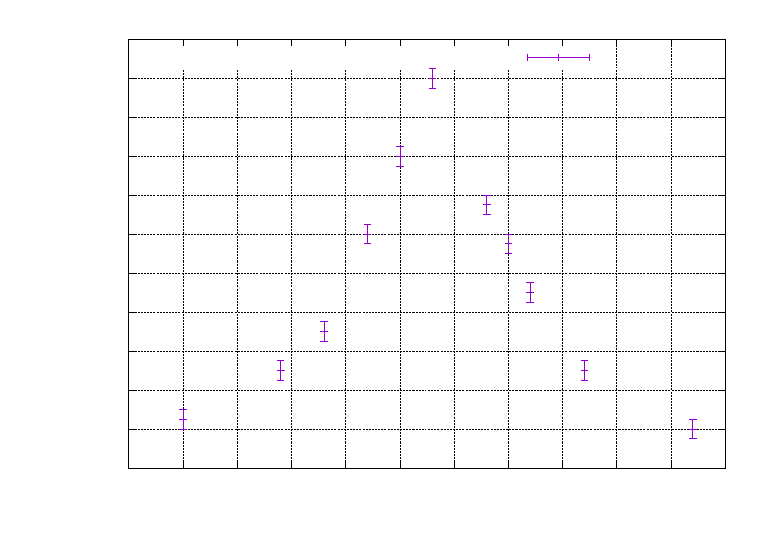
\includegraphics[width={360.00bp},height={252.00bp}]{bilder/resonanzkurve}}%
    \gplfronttext
  \end{picture}%
\endgroup

    \caption{Resonanzkurve}
\end{figure}

\subsubsection{Diskussion}
Die Resonanzkurve hat, wie man sieht eine glockenähnliche Gestalt, welche der Theorie nahe liegt. Bei $f=0,58$(Hz) haben wir den höhsten Wert,
welcher nahe der Eigenfrequenz ist und somit stimmt das mit dem Versuch aus Abschnitt \ref{ssec:eigenfrequenz} überein.

\section{Anhang}
\subsection{Verwendete Geräte}
\begin{itemize}
    \itemsep0em
    \item \quad Bewegungsmesswandler der Firma Leybold, Type 524 082
    \item \quad Software Cassy Lab der Firma Leybold, Type 524 220
    \item \quad Drehpendel nach Pohl der Firma Leybold, Type 34600-B2
\end{itemize}
\listoffigures
\listoftables
\printbibheading[title={Literaturverzeichnis},heading=subbibnumbered]
% \printbibliography[type=book,heading=subbibliography,title={\indent \textit{Bücher}}]
\printbibliography[type=online,heading=subbibliography,title={\indent \textit{Webseiten}}]

\end{document}